\documentclass[aspectratio=169]{beamer}
\title{Buffer Overflows}
\subtitle{Praktische Analyse von Schwachstellen}
\author{Jakob Stühn, John Meyerhoff, Sam Taheri}
\institute{H-BRS}
\usetheme{Berlin}
\setlength{\parindent}{0px}
\newcommand{\alias} [2]{\@ifdefinable #1{\let #1 #2}}
%\alias\realias\let
\newcommand{\providealias}[2]{\@ifundefined #1{\let #1 #2}}

\makeatletter
\newcommand{\fixed@sra}{$\vrule height 2\fontdimen22\textfont2 width 0pt\shortrightarrow$}
\newcommand{\shortarrow}[1]{%
  \mathrel{\text{\rotatebox[origin=c]{\numexpr#1*45}{\fixed@sra}}}
}
\definecolor{method}{rgb}{0.2,0.2,1}
\newcommand{\codeline}[1]{{\color{method}\texttt{#1}}}

%command for z.\,B. ??



\newcommand{\ThesisAuthorGivenName}{}
\newcommand{\ThesisAuthorSurname}{Jakob Stühn, John Meyerhoff, Sam Taheri}
\newcommand{\ThesisAuthor}{\ThesisAuthorSurname}
\newcommand{\ThesisKeywords}{Keywords die diese Arbeit beschreiben}
\newcommand{\ThesisLocation}{Sankt Augustin}
\newcommand{\ThesisPubDate}{7. Januar 2022} %\today
\newcommand{\ThesisSubject}{Schwachstellen und wie man sie Schließt}
\newcommand{\ThesisStudyCourse}{Computer Science}
\newcommand{\ThesisStudyCourseGerman}{Informatik}
\newcommand{\ThesisSubjectType}{Projektbericht}
\newcommand{\ThesisSupervisorFirst}{Mandana Ewert }
\newcommand{\ThesisSupervisorSecond}{Prof. Dr. Stefan Böhmer}
\newcommand{\ThesisTitle}{Buffer Overflow}
\newcommand{\ThesisType}{Bachelor}
\begin{document}

\frame{\titlepage}


\section{Abstract}
Buffer Overflows gehören trotz ihres hohen Alters noch immer zu den relevantesten Schwachstellen in Computerprogrammen.
Aus diesem Grund ist es unabdinglich für jeden, der sich im Feld der Software-Entwicklung oder IT-Sicherheit bewegt, 
ein grundlegendes Verständnis für Buffer Overflows aufzubauen. Ein Überblick über große und aktuelle Angriffe zeigt, 
wie verheerend die Auswirkungen einer solchen Schwachstelle sein können. Ein Buffer Overflow beschreibt im weitesten 
Sinne das “Überlaufen” eines Speicherbereiches durch unvorhergesehene Eingaben, wodurch Schadcode in einen laufenden 
Prozess injiziert und ausgeführt werden kann.

Der vorliegende Projektbericht beschäftigt sich deshalb mit einer theoretisch-technischen Einführung sowie der praktischen 
Analyse von Buffer-Overflow-Schwachstellen. Um eine Grundlage für praktische Tests zu schaffen, wurden zunächst  
die Struktur und der Ablauf eines Programms im Speicher analysiert und theoretische Angriffsmöglichkeiten konstruiert.
Anschließend wurde ein fiktives Angriffsszenario und ein verwundbares C-Programm entwickelt. Hierbei zeigte sich schnell,
dass bereits die Nutzung von vermeintlich harmlosen Funktionen, wie \codeline{fprint()} oder \codeline{gets()}, schwerwiegende Auswirkungen
auf die Sicherheit einer Applikation haben kann. Um die zuvor konstruierten Angriffstechniken real zu erproben und die
Sicht eines Angreifers möglichst realistisch zu analysieren, wurde das verwundbare Programm anschließend im GNU-Debugger
durchleuchtet. Dabei ließ sich klar erkennen, dass der Angreifer von einer Kopie des anzugreifenden Programms, oder sogar
des Source Codes, profitiert. Mit dem aus dem Debugger erlangten Wissen wurde nun ein Exploit gebaut und in einer
simulierten Server-Umgebung ausgeführt. Unter Zuhilfenahme eines injizierten Assembler Programms, konnte auf dem
Zielsystem erfolgreich eine privilegierte Shell geöffnet werden.
Abschließend wurde sich mit den wichtigsten
Abwehrmechanismen auseinandergesetzt und es wurden “cutting-edge” Präventions-Mechanismen,
wie statische Codeanalyse oder Canaries, untersucht. Hier zeigte sich klar,
dass einem Angreifer die Arbeit zwar erschwert werden kann,
Buffer Overflows jedoch nie vollständig verhindert werden können.

Durch diese auf praktische Beispiele fokussierte Herangehensweise soll der Leser dieses Projektberichts die Thematik
der Buffer Overflows besser verstehen und einen direkten Nutzen für seine Arbeit ziehen können.
\pagebreak

\section{Einleitung}
Buffer Overflows sind toll..............

\pagebreak

% Sam:
\section{Geschichte}
\subsection{Bekannte Buffer Overflows}
Es folgen Beispiele für historische sowie aktuelle Angriffe auf der Grundlage von Buffer Overflows:

„The Morris Worm“ der am 2. November 1988 ins damals noch junge Internet freigelassen wurde und sich rasant verbreitete,
verursachte großen Schaden in Form von überlasteten Systemen und Totalausfällen. Der Wurm wurde vom amerikanischer Robert T. Morris in C geschrieben
und umfasste ca. 3200 Programmierzeilen. Morris war Student an der Cornell University und wollte mit seinem Programm die angeschlossenen Rechner an einem Netz zählen.
Stattdessen legte er nach nur 15 Stunden 10\% des damaligen Internets lahm. Morris wurde zu drei Jahren Haft und einer Geldstrafe von 10.000 US-Dollar verurteilt. \cite{wiki1}

Ein weiteres historisches Beispiel ist der „SQL-Slammer“. Dieser wurde am 25. Januar 2003 entfesselt und hatte schon innerhalb von 30 Minuten über 75.000 Opfer.
Der Computerwurm infizierte ungepatchte Microsoft SQL Server 2000 und nutze dabei zwei Buffer Overflow Schwachstellen.
Das Besondere an diesem Wurm war seine kompakte Größe: Er bestand aus einem UDP-Paket von lediglich 376 Bytes und bewegte sich ausschließlich im Arbeitsspeicher des befallenen
Computers, nicht jedoch auf der Festplatte. Der Wurm lieferte dabei keinerlei Payload, sondern versuchte lediglich sich selbst zu kopieren und
so viele Computer wie möglich zu infizieren. Bei den Entwicklern handelte es ich um zwei Mitglieder der Gruppe 29A, die im Jahr 2004 gefasst wurden. \cite{wiki2}

Eine aktuellere Schwachstelle fand sich 2019 im Messenger Dienst WhatsApp. Diese ermöglichte es Angreifern,
mit der Hilfe von manipulierten Videodateien Malware einzuschleusen und sich so Zugriff auf Smartphones zu verschaffen.
Die Sicherheitsabteilung von Facebook sprach von einem „Stack-based Buffer Overflow“ der über korrupte MP4-Dateien ausgenutzt wurde.
Der Fehler wurde durch einen Patch behoben. \cite{whatsapp1}

Beim letzten Beispiel handelt es sich um eine Sicherheitslücke in HP-Druckern.
Dabei dreht es sich konkret um zwei Sicherheitsprobleme in der Firmware von HP, von der viele Druckermodelle betroffen sind.
Eine Liste dieser wurde bereits veröffentlicht. Die Sicherheitslücken erlauben dem Angreifer durch veränderte Anfragen an den Drucker einen Buffer Overflow auszulösen
und Schadcode zu injizieren. Die Lücken wurden mittlerweile durch ein Update geschlossen, es existieren jedoch immer noch viele anfällige Systeme. \cite{hpvuln}

\pagebreak

% Jakob:
\section{Grundlegende Theorie}
\subsection{Definition}
Im weitesten Sinne beschreibt ein Buffer Overflow eine Schwachstelle in einem Computerprogramm,
bei der ein Angreifer einen Speicherbereich fester Größe überschreibt und diesen so zum “Überlaufen” bringt.
Durch Ausspähen und Analysieren der Software kann dieses Überschreiben so gezielt geschehen, dass der Fluss des
Programms verändert und zuvor injizierter Schadcode ausgeführt wird. \cite{NISTSP} \cite{springer}
\subsection{Speicheraufbau}
Wird eine Binärdatei durch den Linker von der Festplatte entnommen, so wird der auszuführende Programmcode
zunächst in den Arbeitsspeicher geladen. Im Speicher gliedert sich der Prozess dann in folgende Segmente:
\begin{itemize}
    \item \textbf{Stack}: Wächst von oben nach unten und enthält lokale Daten sowie Funktionsparameter
    \item \textbf{Heap}: Wächst von unten nach oben und enthält dynamisch allozierten Speicher
    \item \textbf{Data}: Liegt unter dem Heap und enthält initialisierte statische Variablen
    \item \textbf{Text}: Liegt unter dem Data-Segment und enthält die Assembler-Instruktionen des Programms
\end{itemize}

(Segmente, die im weiteren Verlauf keine größere Rolle spielen, werden hier unterschlagen.)
\begin{figure}[h]
    \centering
    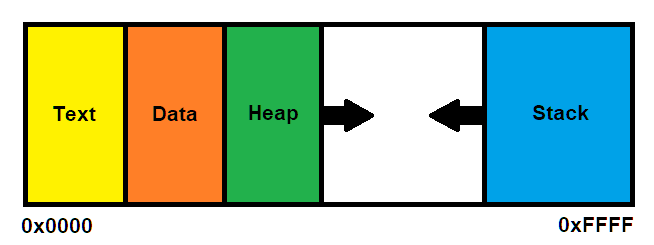
\includegraphics[width=0.7\textwidth,height=0.75\textheight,keepaspectratio]{images/process.png}
    \caption{Prozess im Speicher}
\end{figure}

Wenn eine Funktion aufgerufen wird, legt diese zunächst ihre Funktionsparameter auf den Stack,
gefolgt von einer Return-Adresse, die angibt, zu welcher Stelle im Programm im Anschluss an die
Ausführung der Funktion gesprungen wird, und einem Base Pointer. Darauf folgen lokale Daten,
die von der Funktion verwendet werden, wie z.\,B. ein Char Array. \cite{hamburg}
\pagebreak
\subsection{Stack Overflow} \label{sec:stackoverflow}
Der zuvor beschriebene Aufbau des Stacks lässt sich nun durch gezieltes Einfügen von Daten in eine Funktion ausnutzen.
Wenn beispielsweise ein Char Array mit einer Größe von 64 Bytes auf den Stack gelegt wird und es dem Angreifer gelingt,
als Folge von fehlerhafter Programmierung eine Zeichenkette mit mehr als 64 Bytes in das Array zu laden, so können
die überschüssigen Zeichen andere Daten im Stack überschreiben. Durch diese Methode kann der Prozess auf folgende
Weisen beeinflusst werden:
\begin{itemize}
    \item Es kann der Wert einer Variable verändert werden, um den Prozess zu manipulieren.
    \item Function Pointer können manipuliert werden, um den Programmfluss umzuleiten und zuvor präparierten Shellcode auszuführen.
    \item Auch durch das Überschreiben von Return Pointern kann auf Shellcode umgeleitet werden.
\end{itemize}

Ausgeführter Shellcode läuft dann immer unter denselben Privilegien wie der Prozess. \cite{cloudflare} \cite{fortinet}
\begin{figure}[h]%
    \centering
    \subfloat[\centering Vorher]{{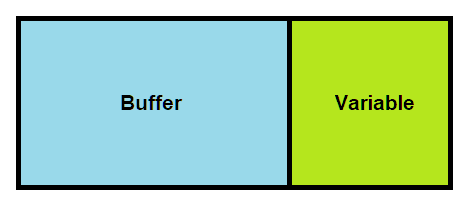
\includegraphics[width=0.45\textwidth,height=0.75\textheight,keepaspectratio]{images/buffer1.png} }}%
    \qquad
    \subfloat[\centering Nachher]{{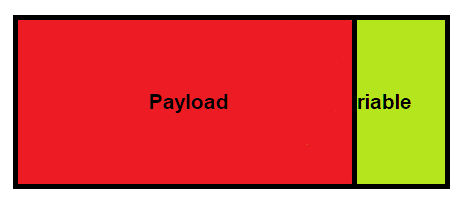
\includegraphics[width=0.45\textwidth,height=0.75\textheight,keepaspectratio]{images/buffer2.png} }}%
    \caption{Buffer im Stack während eines Overflows}%
    \label{fig:example}%
\end{figure}

\subsection{Heap Overflow} \label{sec:heapoverflow}
Während der Laufzeit eines Programms allozierter Speicher (z.\,B. durch \codeline{malloc()}) wird im Heap angelegt. Dabei setzt sich
jeder Speicherblock aus einem Header und dem tatsächlich angeforderten Speicher zusammen. Der Header enthält hierbei,
je nach Implementation, Informationen über den Block, wie z.\,B. seine Größe. Aus diesen Informationen kann dann abgeleitet
werden, an welcher Stelle der nächste Block beginnt.

Wenn ein Angreifer nun Manipulationen im Heap-Speicher vornehmen möchte, muss er die verwendete Implementation kennen
und kann in der Regel nur in Richtung der neu allozierten Speicherblöcke überschreiben. Da er aus dem Heap keine Möglichkeit
hat, Sprungadressen direkt zu manipulieren und den Programmfluss so umzuleiten, muss er versuchen, einen bestimmten
Speicherblock zu überschreiben, zu dem im weiteren Programmverlauf noch einmal gesprungen wird. Dies macht Heap Overflows
in der Praxis um einiges komplexer und schwieriger als Stack Overflows. \cite{heise}




% Sam:
\section{Shellcode}
\subsection{Definition}
Um den nächsten Teil besser zu verstehen, sollte vorher erklärt werden, was genau Shellcode ist, wofür er 
benutzt wird und was der Zusammenhang zur Assembler Programmiersprache ist. Shellcode ist definiert als eine 
Reihe von Anweisungen, die über einen Exploit injiziert und dann durch den Prozess ausgeführt werden.
Shellcode wird verwendet, um Register direkt zu manipulieren und die Funktionalität eines Programms auszunutzen. 
Es ist natürlich möglich, Shellcode in höheren Programmiersprachen zu schreiben, aber die effizienteste und fast 
ausschließlich benutzte Variante ist in der Sprache Assembly, die so maschinennah wie möglich ist, um genau steuern 
zu können was passiert und Speichergröße zu sparen. Meistens arbeitet man nämlich mit einer limitierten Speichergröße.
In der Computersicherheit bedeutet Shellcoding im wahrsten Sinne des Wortes das Schreiben von Code, der bei der
Ausführung eine Remote-Shell zurückgibt. Die Bedeutung von Shellcode hat sich weiterentwickelt und stellt nun jeden
Byte-Code dar, der in einen Exploit eingefügt wird, um eine gewünschte Aufgabe zu erfüllen. Da Shellcode in Assembly
geschrieben wird und die Sprache so maschinennah wie nur möglich ist, ist es außerdem noch wichtig mit welcher
Hardware und mit welchem Betriebssystem man diese schreibt. Es bestehen nämlich Unterschiede zwischen Linux
Shellcode und Windows Shellcode:  Bei Linux hat man direkten Zugriff auf das Interface und das Kernel, was bei
Windows leider nicht möglich ist. Im folgenden Beispiel wird ein Shellcode-Beispiel in der Sprache Assembly erläutert.
Die Idee hinter dem Beispiel ist es, zu zeigen, wie man mit einem Buffer Overflow Zugriff bekommen kann und dann den
vorbereiteten Shellcode injizieren kann, damit dieser privilegiert ausgeführt wird und somit Schaden am Ziel verursacht.

\subsection{Beispiel}
\begin{figure}[h]
    \centering
    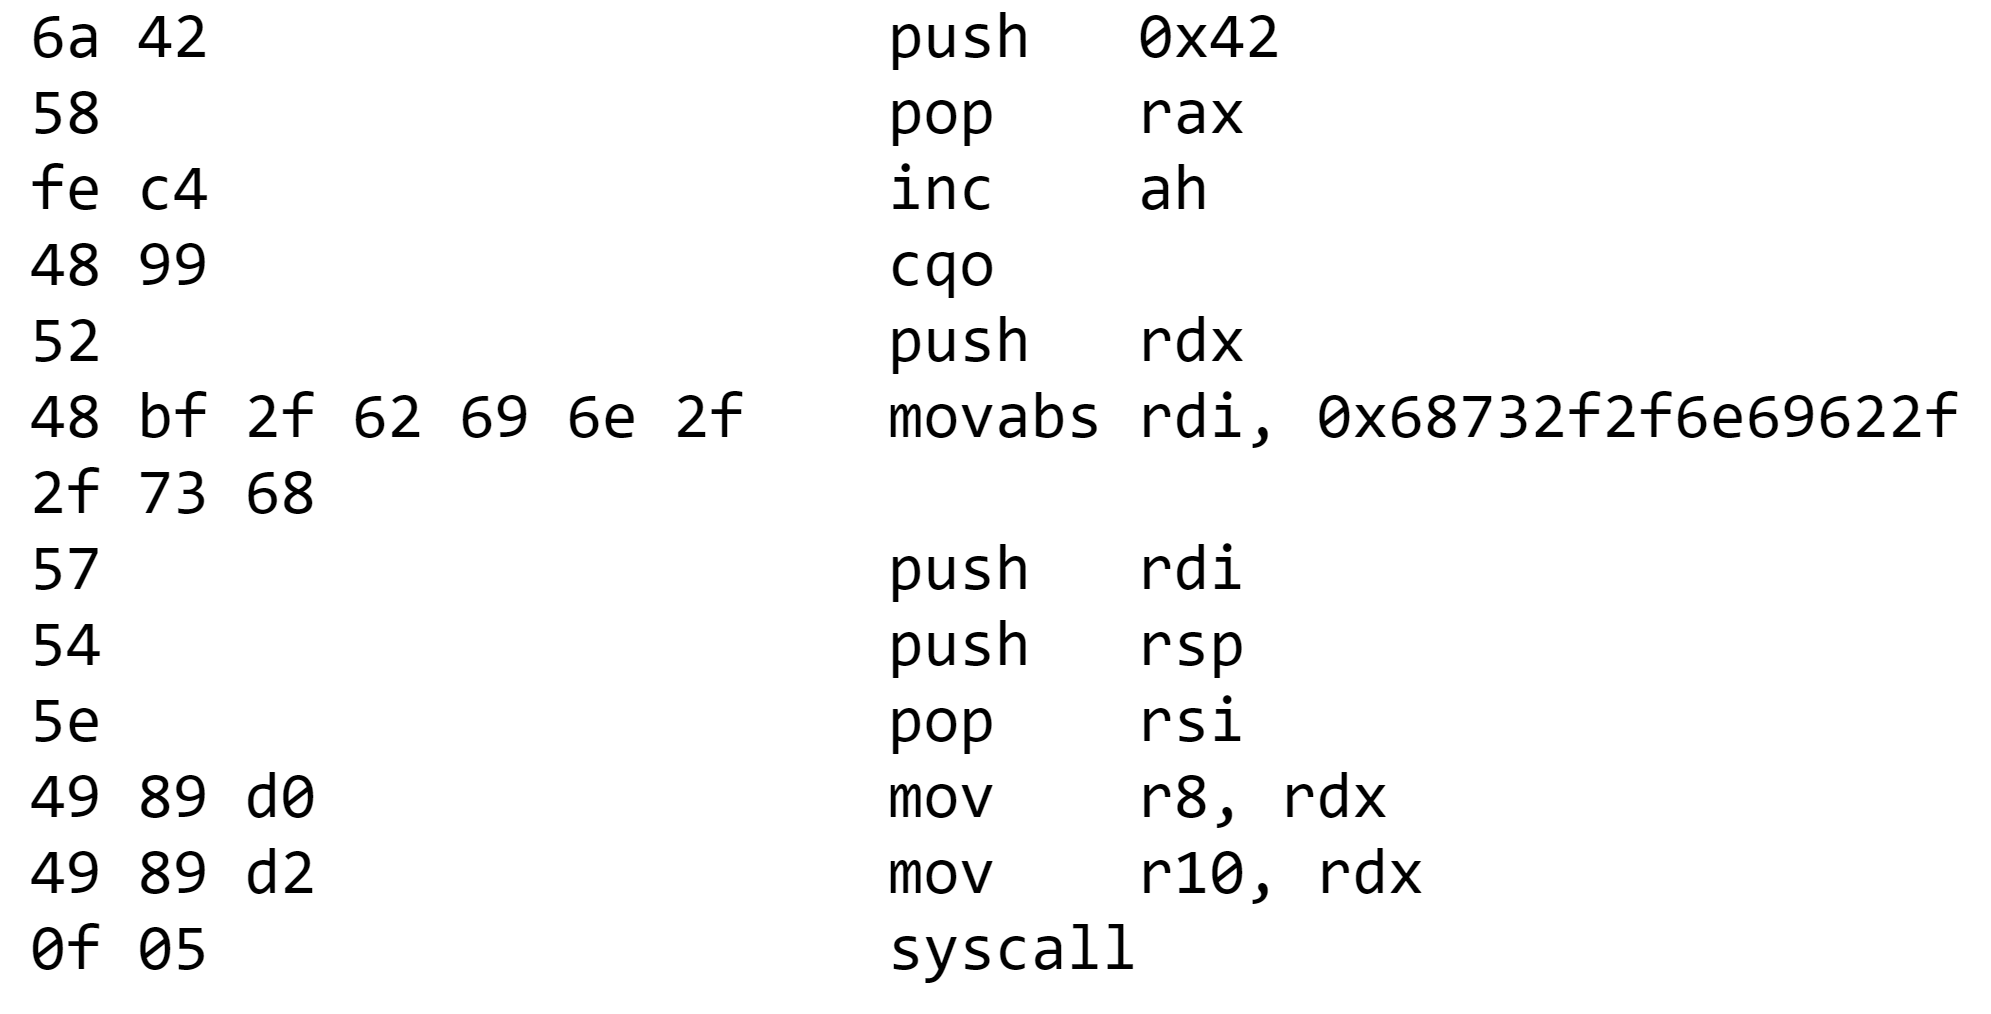
\includegraphics[width=0.9\textwidth,height=0.75\textheight,keepaspectratio]{images/shellstorm.png}
    \caption{Shellcode}
\end{figure}

%TODO: Einfügen aus DC
%Struktur:
%Der syscall wird abgeschickt, vorher müssen einige Werte gesetzt werden um execveat aufzurufen



RAX -> system call number (322) 
RDI -> first argument (path)
RSI -> second argument (pointer to path)
RDX -> third argument (0)
R10 -> fourth argument(0)
R8 -> fifth argument(0)
R9 -> sixth argument (not used) (Bearbeitet)


Bei dem folgenden Bild sieht man ein Beispiel zu einem Shellcode der dann wenn man
%!!!
vorhat ausgeführt werden kann um ein System zu manipulieren.Dieses ist aber einfach
gehalten um einen übersichtlicheren Blick zu bekommen. Daher sollte man hier von unten
beginnen. Der System Call wird aufgerufen und geht an die Adresse im Register RAX.
Dieser wurde mit der Hexadezimalzahl 0x42 belegt die auf den Stack gepusht
war und durch das pop da eingespeichert wurde, wichtig hierbei ist dass,
danach das Register ah was ein 8 Bit Teil vom 64 Bit Register RAX ist inkrementiert wird.
Mit anderen Worten wird der Wert 0x42 zum Wert 0x142 dieser ist in
Dezimalzahlen 322.Also geht der  System Call an die Nummer 322.
Der nächste Schritt des Aufrufs ist es ans Register RDI zu gehen was das first
argument enthält und den path darstellt. Im Code sehen wir das durch den
Befehl movabs der String ("/bin//sh") als Hexadezimalzahl ins Register
verschoben wird und danach durch den push Befehl auf dem Stack ist.
Der dritte Schritt ist dass, der Aufruf sich das second argument anguckt
was den Weg zum path hat und im Register RSI enthalten ist. Das besondere
Register RSP oder auch stack pointer zeigt auf den Pfad der letzten Adresse
in dem falle den von RDI und dieser Pfad wird in RSI gespeichert, daher die
Befehle push RSP und pop RSI. Der Rest vom Code ist in diesem falle nicht so
wichtig aber durch den Befehl cqo(convert word to Quadword) am Anfang wird das
Register RDX auf null gesetzt und diesen Wert übernehmen dann auch die zwischen
Register R8 und R10 durch den mov Befehl. Einen wirklichen nutzen hat dieser
kleine 29 Byte große
Shellcode nicht, aber er zeigt hervorragend wie man die Register mit dem der
Kernel durch den System Call arbeitet man manipulieren kann.

\pagebreak

\begin{frame}{Praktische Analyse}{Programmierfehler}
    Overflow-anfällig sind Sprachen, welche direkte Zugriffe auf die Speicherstrukturen\\ des Systems ermöglichen:
    \begin{itemize}
        \vspace{1em}
        \item Assembly
        \item C/C++
        \item Fortran
    \end{itemize}
\end{frame}

\begin{frame}{Praktische Analyse}{Programmierfehler}
    Problematisch sind Funktionen, welche
    keine Kontrolle auf die Länge des Inputs implementieren: %ausüben / durchführen
    \begin{itemize}
        \vspace{1em}
        \item \codeline{gets(buffer)}\\ Erwartet Input und kopiert diesen in den angegebenen Speicher
        \vspace{1em}
        \item \codeline{strcopy(buffer, input)}\\ Kopiert einen Input
        in den angegebenen Speicher
    \end{itemize}
\end{frame}


\begin{frame}{Praktische Analyse}{Format-String-Schwachstelle}
    Unvorsichtige Verwendung von Formatierungsfunktionen:
    \begin{itemize}
        \vspace{1em}
        \item \codeline{printf(``\%s'', chars)}\\ Korrekte/Sichere Verwendung
        \vspace{1em}
        \item \codeline{printf(chars)}\\ Falsche/Unsichere Verwendung
    \end{itemize}
%BIG CODEIMAGE
\end{frame}

\begin{frame}{Praktische Analyse}{Demonstration}
    \begin{figure}[h]
        \centering
        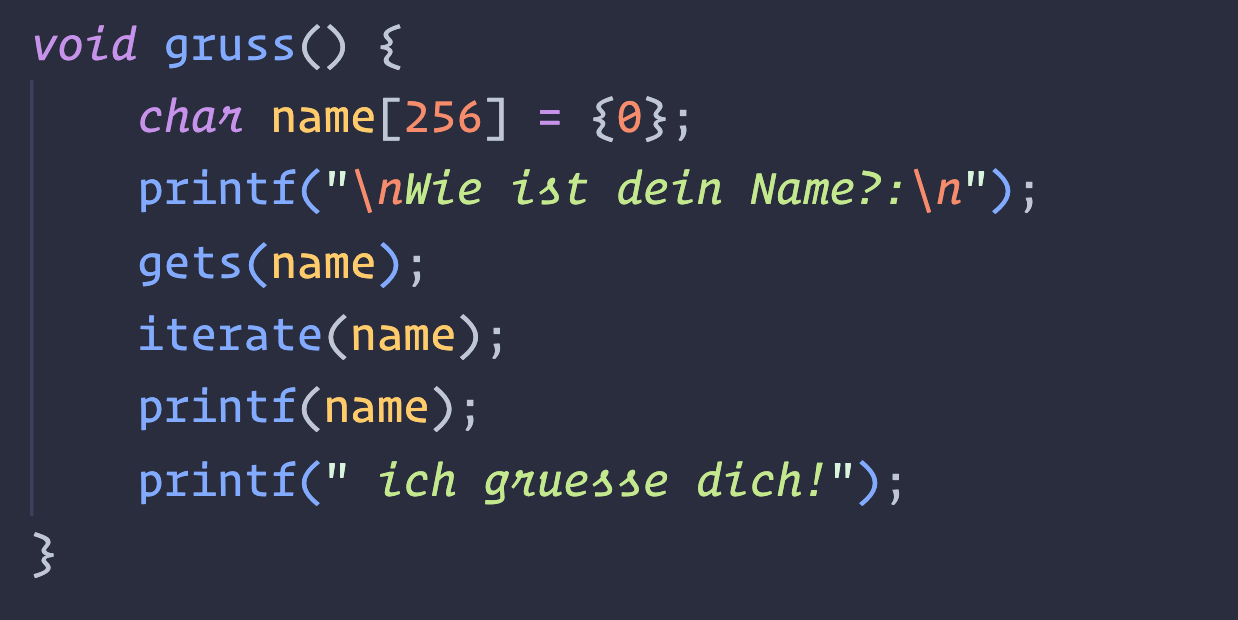
\includegraphics[width=0.7\textwidth,height=0.75\textheight,keepaspectratio]{images/gruss.png}
        \caption{Funktion \codeline{gruss()} }
    \end{figure}
\end{frame}

\begin{frame}{Praktische Analyse}{Demonstration}
    \begin{figure}[h]
        \centering
        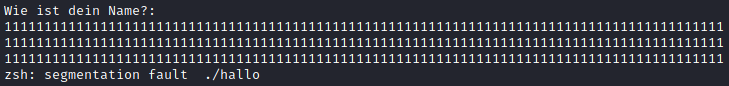
\includegraphics[width=0.7\textwidth,height=0.75\textheight,keepaspectratio]{images/segfault.png}
        \caption{Segmentierungsfehler}
    \end{figure}
    \begin{figure}[h]
        \centering
        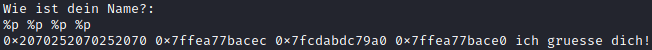
\includegraphics[width=0.7\textwidth,height=0.75\textheight,keepaspectratio]{images/adressen.png}
        \caption{Ausgegebene Speicheradressen}
    \end{figure}
\end{frame}

\begin{frame}{Praktische Analyse}{Demonstration}
    \begin{figure}[h]
        \centering
        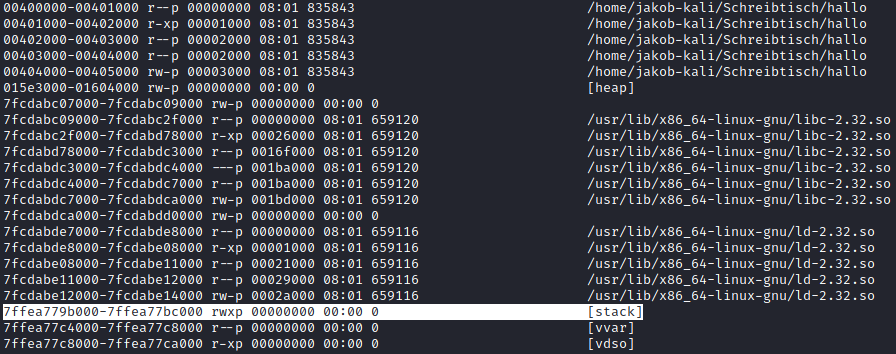
\includegraphics[width=0.7\textwidth,height=0.75\textheight,keepaspectratio]{images/map.png}
        \caption{Memory Map}
    \end{figure}
\end{frame}

\begin{frame}{Praktische Analyse}{Demonstration}
    \begin{figure}[h]
        \centering
        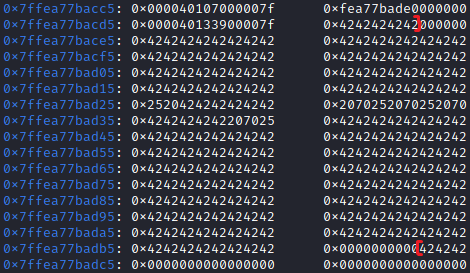
\includegraphics[width=0.7\textwidth,height=0.75\textheight,keepaspectratio]{images/buffer.png}
        \caption{Speicherinhalt}
    \end{figure}
\end{frame}

\begin{frame}{Praktische Analyse}{Demonstration}
    \begin{figure}[h]
        \centering
        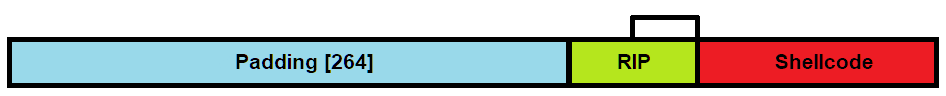
\includegraphics[width=0.7\textwidth,height=0.75\textheight,keepaspectratio]{images/payload1.png}
        \caption{Payload 1}
    \end{figure}
    \begin{figure}[h]
        \centering
        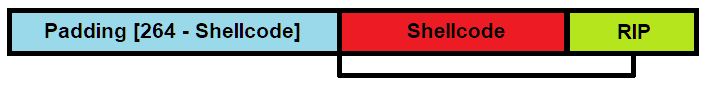
\includegraphics[width=0.7\textwidth,height=0.75\textheight,keepaspectratio]{images/payload2.png}
        \caption{Payload 2}
    \end{figure}
    \begin{figure}[h]
        \centering
        
\includegraphics[width=0.5\textwidth,height=0.75\textheight,keepaspectratio]{images/nop.png}
        \caption{NOP Slide}
    \end{figure}
\end{frame}

\begin{frame}{Praktische Analyse}{Demonstration}
    \begin{figure}[h]
        \centering
        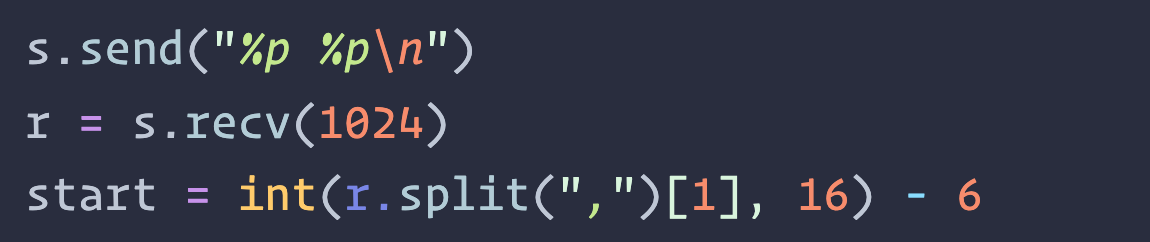
\includegraphics[width=0.5\textwidth,height=0.75\textheight,keepaspectratio]{images/format.png}
        \caption{Format-String-Ausgabe}
    \end{figure}
    \begin{figure}[h]
        \centering
        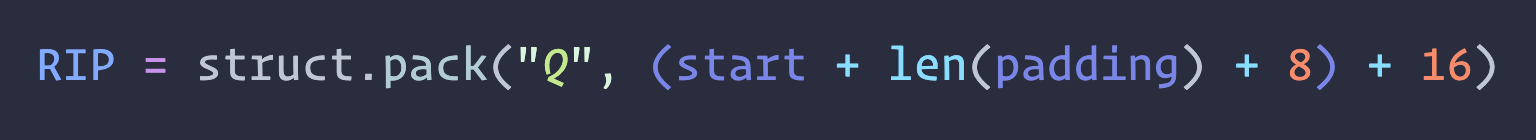
\includegraphics[width=0.5\textwidth,height=0.75\textheight,keepaspectratio]{images/rip.png}
        \caption{RIP}
    \end{figure}
    \begin{figure}[h]
        \centering
        
\includegraphics[width=0.5\textwidth,height=0.75\textheight,keepaspectratio]{images/payload.png}
        \caption{Payload}
    \end{figure}
\end{frame}

\begin{frame}{Praktische Analyse}{Demonstration}
    \begin{figure}[h]
        \centering
        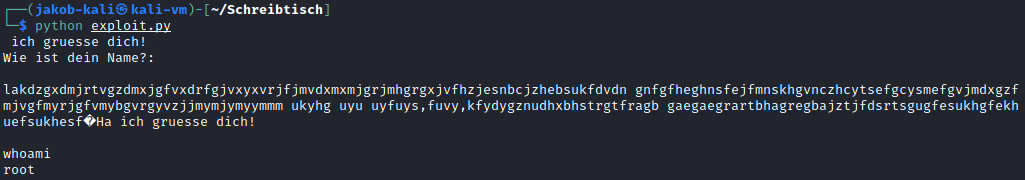
\includegraphics[width=0.8\textwidth,height=0.75\textheight,keepaspectratio]{images/root.png}
        \caption{Root Shell}
    \end{figure}
\end{frame}



% Jakob:
%\section{Praktische Analyse}


\subsection{Programmierfehler}
Grundsätzlich kann jede Software von Buffer Overflows betroffen sein, die in einer Programmiersprache geschrieben ist, 
welche direkte Zugriffe auf die Speicherstrukturen des Systems ermöglicht. Beispiele hierfür wären: Assembler, C/C++ oder 
Fortran. Prinzipiell nicht betroffen sind Programme, die in einer interpretierten Sprache wie Python oder Java geschrieben 
sind. Bei diesen Sprachen wäre nur ein Overflow im Interpreter selber möglich, da dieser in der Regel auf einer der zuerst 
genannten Sprachen basiert.

Am problematischsten sind hierbei Funktionen, die es ermöglichen Nutzereingaben zu lesen und zu speichern,
die jedoch nicht die Länge der eingegebenen Daten überprüfen können. Zwei der bekanntesten Vertreter für Funktionen
dieser Art sind die C Funktionen \codeline{gets()} und \codeline{strcopy()}:
\begin{itemize}
    \item \codeline{gets(buffer)} Fragt nach Input und kopiert die Eingaben in den angegebenen Speicher
    \item \codeline{strcopy(buffer, input)} Kopiert den Input (z.\,B. ein Kommandozeilenargument)\\ in den angegebenen Speicher
\end{itemize}
Da keine Kontrolle auf die Länge des Inputs durchgeführt wird, kann nicht sichergestellt werden,
dass der angegebene Speicherbereich ausreichend groß ist oder ob der Input in andere Bereiche überläuft.

\subsection{Format-String-Schwachstelle}
Bei Format-String-Schwachstellen handelt es sich zwar nicht direkt um eine Art von Buffer Overflow,
jedoch können diese oft in ähnlichen Kontexten aufkommen und ermöglichen es Angreifern, 
Informationen über die Interna eines Programms zu gewinnen. 

Problematisch ist hierbei die unvorsichtige Verwendung von Formatierungsfunktionen wie \codeline{fprint()}.
Soll beispielsweise eine Zeichenkette ausgegeben werden, sollte korrekterweise ein Formatierungsparameter
wie \codeline{\%s} verwendet werden: \codeline{printf(“\%s”, chars)}. Die Unterschlagung dieses Parameters 
scheint zwar auf den ersten Blick dasselbe Ergebnis zu liefern: \codeline{printf(chars)}. Die zweite Variante ermöglicht
es dem Angreifer jedoch, eigene Parameter einzusetzen, um Informationen auszulesen oder zu manipulieren:
\begin{itemize}
    \item \codeline{\%x} Liest Daten vom Stack
    \item \codeline{\%s} Liest Strings aus dem Prozess
    \item \codeline{\%n} Schreibt einen Integer in den Prozess
    \item \codeline{\%p} Gibt Pointer auf void aus
\end{itemize}


\subsection{Code}
\subsection{Setup des Servers}
\subsection{Böswilliger Client}
\subsection{Erläuterung des Vorgangs} \label{explainersub}
% John:
\section{Gegenmaßnahmen}
Wie in Abschnitt \ref{sec:explainersub} bereits aufgeführt,
gehören zu einem Buffer-Overflow-Angriff mehrere kombinierte Teile. Wenn
man nun verhindern möchte, dass ein Programm über diesen Angriff gestürzt werden
kann, so hat man mehrere Möglichkeiten diese Teile aufzuhalten oder die Kombination
zu blockieren. Es folgen mehrere Möglichkeiten, grob nach Aufwand (für den Entwickler) sortiert.
\subsection{Übersicht der Maßnahmen}
Low-Level:
    \begin{itemize}
        \item Hardware-basierte Lösungen
        \item Betriebssystembasierte Ansätze
    \end{itemize}
Passive Härtung der Programme:
    \begin{itemize}
        \item C Range Error Detector und Out Of Bounds Object
        \item Safe Pointer Instrumentalisierung
        \item Manuelles Buffer-Overflow Blocken (Input-Bereinigung)
    \end{itemize}
Aktive (Analysierende) Lösungen:
    \begin{itemize}
        \item Statische Code-Analyse
        \item Stack-Schutz mit ``Canary'' (Zufallszahl)
    \end{itemize}


\subsection{Low-Level Probleme}
Sowohl Hardwarelösungen als auch Betriebssystembasierte Lösungen haben
das grundlegende Problem, dass die Verhinderung von Buffer-Overflows zu
ungewünschten Nebeneffekten führen kann. Es ist auf jeden Fall möglich,
jegliche Overflows zu verhindern - dabei werden jedoch auch vom
Entwickler gewünschte Overflows verhindert, sodass Programme nicht mehr
ordentlich funktionieren. Manchmal wird aus gründen der Effizienz ein
Buffer zum Überlaufen gebracht, ohne dass dieser Überlauf unkontrolliert
ist. Leider ist es Praktisch nicht umsetzbar, in einer Hardwarelösung
zu entscheiden, welcher Buffer-Overflow böswillig ist.



\subsection{Out Of Bounds Object}
Ein Out Of Bounds Object ist eine Vereinfachte Lösung um Referenzen ungefährlich zu machen.
Es wird verhindert, dass auf Speicher außerhalb des Programms zugegriffen wird, indem Jede
Adresse welche nicht im spezifizierten Bereich liegt auf ein bestimmtes Objekt, das sogenannte
"Out Of Bounds Object" verweist. Dadurch kann innerhalb des laufenden Programms erkannt werden, das
etwas falsch gelaufen ist. Diese Methode ist nicht gängig, da sie technisch gesehen
umgangen werden kann, solange der Angreifer weiß, welcher Speicherbereich für das Programm
vorgesehen ist.

\subsection{Statische Analyse}
Wenn das Programm bereits vor der Ausführung analysiert wird, kann ein
Tool bestimmen, an welchen stellen Schwachstellen vorhanden sind und
ggf. vorschlagen, wie diese behoben werden können. Leider ist bei größeren
Projekten die Aussage, dass keine Schwachstellen mehr vorhanden seien
unmöglich zu treffen.

\subsection{Canaries}
Die Bezeichnung Canary (Engl. Kanarienvogel) stammt aus der Verwendung der Kanarienvögel als
Indikator für Gas in Mienen. Die Canaries im Code werden als Stack-Schutz verwendet. Das bedeutet,
dass beispielsweise Zufallszahlen im Programm auf dem Stack sind und bei einem Buffer-Overflow-Angriff
überschrieben werden. Ein Tool wie StackGuard kann dann anhand der Änderung einen Fehler feststellen und
die Ausführung des Programms abbrechen.

%TODO: ASLR Beschreiben

\subsection{Code-Beispiel}
    \begin{center}
        %TODO: Besseres Beispiel finden.
        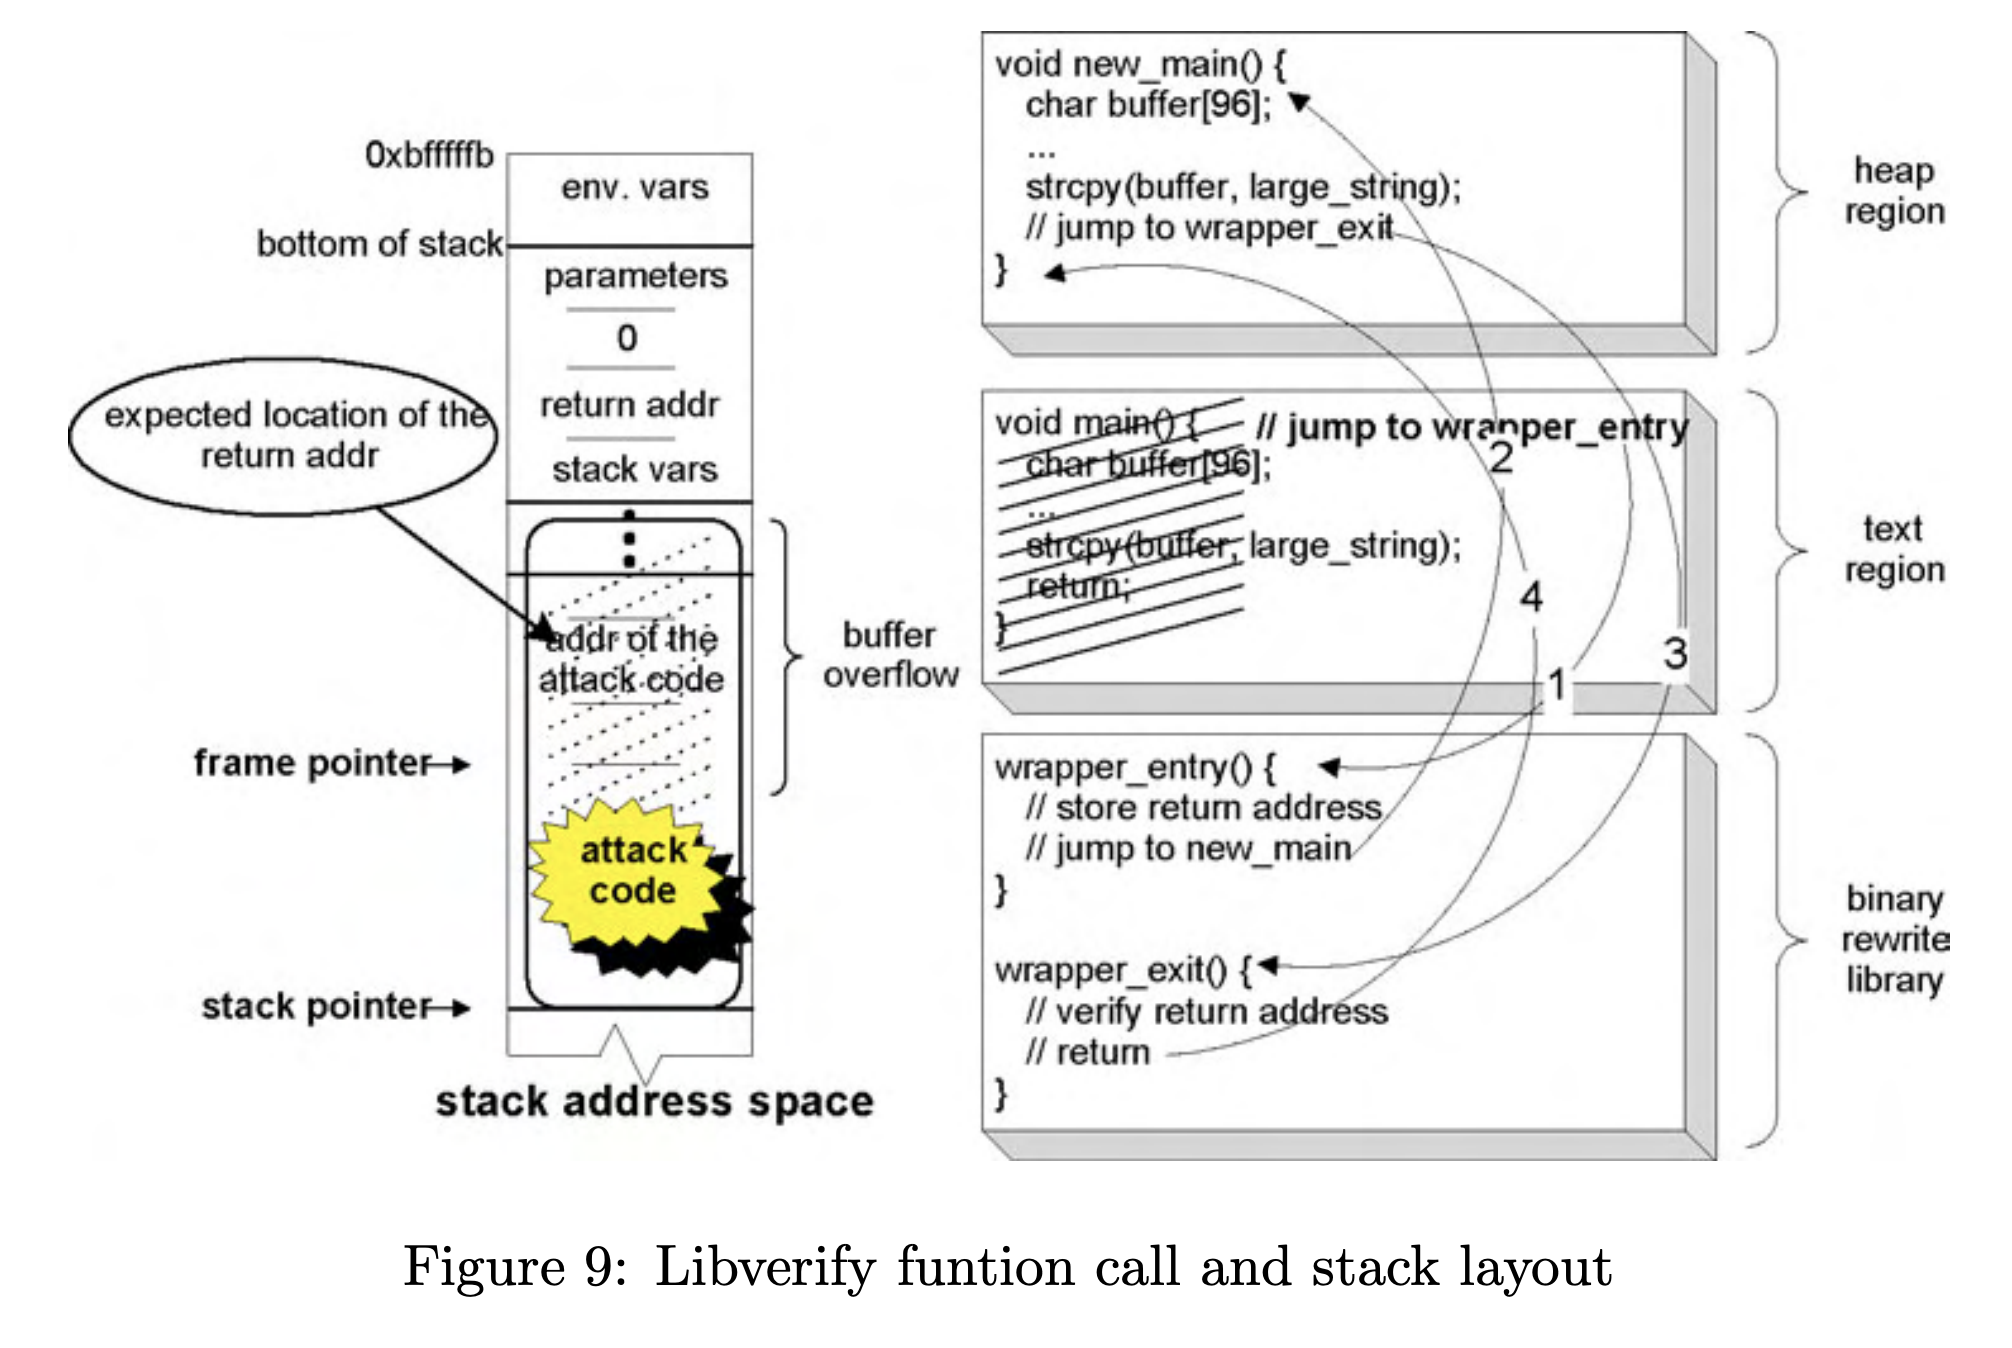
\includegraphics[width=\textwidth,height=0.75\textheight,keepaspectratio]{images/Libverify.png}
    \end{center}

\subsection{Testen}
Es gibt mehrere Möglichkeiten um kompilierte Programme auf ihre Sicherheit
und Robustheit zu testen. Diese beiden Qualitätsmerkmale sind vor Allem
im Bezug zu Buffer-Overflows am wichtigsten. Wartbarkeit und Erweiterbarkeit
sind langfristig auch zu beachten, da es bei Änderungen am Quellcode
zu Fehlern kommen kann, welche Schwachstellen herbeibringen.
Mit Werkzeugen wie Sonar lint können vor allem häufig auftretende Fehler entdeckt
werden.
%Beispielkommentar
Im Bereich der Overflow Payloads gibt es mehrere Werkzeuge um Fuzzy Testing
zu betreiben. Beim Fuzzy Test wird strukturiert zufällig auf eine 
potentielle Schwachstelle getestet, wobei die tatsächlichen aufrufe
von einem sogenannten Fuzzer erstellt werden.
Als Alternative zum Fuzzing gibt es Spezifische Payloads und
Escape-Sequenzen welche - auch automatisiert - getestet werden können.



%Everybody <3
\pagebreak

\section{Fazit}
Dadurch dass es diverse Angriffsmöglichkeiten und Gegenmaßnahmen gibt,
ist es sowohl für Angreifer als auch Angriffsziel nicht einfach,
eine Übersicht über die offenen Schwachstellen eines Prozesses zu halten.

\cite{phrack}
\cite{computerphile}
\cite{protostar}
%\section{Quellen}
    \begin{itemize}
        \item https://www.nds.ruhr-uni-bochum.de/media/nds/attachments/files/2010/11/Survey.on.Buffer.Overflow.Attacks.and.Countermeasures.pdf
    \end{itemize}

\end{document}
